\documentclass{article}
\pagenumbering{arabic}
\newcommand{\newCommandName}{text to insert}
% Pages and colors used for the cover page
\usepackage{tikz-page}
\usepackage{url}
\usepackage{lastpage}

% Used for the math and code
\usepackage{amsmath}
\usepackage{listings}
\usepackage{pythonhighlight} % Got this from github! https://github.com/olivierverdier/python-latex-highlighting/blob/master/pythonhighlight.sty

% Used for the pictures
\usepackage{float}
\usepackage{graphicx}

% For the table
\usepackage[utf8]{inputenc}
\usepackage{multirow}
\usepackage{colortbl}

\usepackage[
  top=2cm,
  bottom=2cm,
  left=3cm,
  right=2cm,
  headheight=17pt, % as per the warning by fancyhdr
  includehead,includefoot,
  heightrounded, % to avoid spurious underfull messages
]{geometry} 

% Page numbers/header
\usepackage{fancyhdr}
\definecolor{brickred}{rgb}{0.8, 0.25, 0.33}
\definecolor{cobalt}{rgb}{0.0, 0.28, 0.67}
\definecolor{cadetgrey}{rgb}{0.57, 0.64, 0.69}

% Defining the text box being used for DEPT OF ENG
\tikzset{
        secnode/.style={
                minimum height = .16in,
                minimum width = 4.16in,
                inner xsep = 2pt,
                anchor=north east,
                draw=cadetgrey,
                fill=white,
                text=brickred,
                },
        }


         
\pagestyle{plain}
\renewcommand{\headrulewidth}{0pt}
\begin{document}


% Put name data and assignment number here
\newcommand\personaldate{February 27, 2024}
\newcommand\myname{Leo Berman}
\newcommand\myemail{leo.berman@temple.edu}
\newcommand\hwnum{04}
\newcommand\mynameabbrev{L. Berman}
\newcommand\assignmenttitle{Gaussian Mixture Distribution Parameter Estimation}
\newcommand\yourclass{ECE 8527: Machine Learning and Pattern Recognition}
\begin{titlepage}
	% Drawing the border and the text box 
	\newcommand{\tikzpagelayout}{
		\draw[line width = .04in,
			color = cobalt]
		($(current page.north west)+(1in,-1in)$)
		rectangle ($(current page.south east)+(-.625in,1in)$);

		\draw[line width = .04in,
			color = brickred]
		($(current page.north west)+(.92in,-.92in)$)
		rectangle ($(current page.south east)+(-.705in,1.08in)$);
		\node[secnode] at ($(current page.north west)+(6in,-.875in)$) {\small{\textbf{DEPARTMENT OF ELECTRICAL AND COMPUTER ENGINEERING}}};
	}

	\begin{center}
		\large{Homework Assignment No. \hwnum:}\break
		\break
		\large{\textbf{HW No. \hwnum: \assignmenttitle}}\break
		\break
		\large{submitted to \:}\break
		\break
		\large{Professor Joseph Picone}\break
		\large{ECE 8527: Introduction to Pattern Recognition and Machine Learning}\break
		\large{Temple University}\break
		\large{College of Engineering}\break
		\large{1947 North 12th Street}\break
		\large{Philadelphia, Pennsylvania 19122}\break
		\break
		\large{\personaldate}\break
		\break
		\large{prepared by: }\break
		\break
		\large{\myname}\break
		\large{Email: \myemail}
	\end{center}
\end{titlepage}

\newpage
\pagestyle{fancy}
\fancyhead{}
\fancyfoot{}
\fancyhead[R,EH]{Page \thepage\ of \pageref{LastPage}}
\fancyhead[L,EH]{\mynameabbrev: HW \# \hwnum}
\fancyfoot[L,EF]{\yourclass}
\fancyfoot[R,EF]{\personaldate}
\renewcommand{\thesection}{\Alph{section}.}

\section{\MakeUppercase{Generate Data and plot a single component Gaussian mixture model}}
In terms of the nature of the fit seen below, it's clear that a single component Gaussian distribution is insufficient for representing this dataset. There are clearly 3 peaks which represent the three means. The reason the middle peak is largest is due to the variance of the other sets overlap.
\begin{figure}[!htb]
	\centering
	\begin{minipage}{0.49\textwidth}
			\centering
			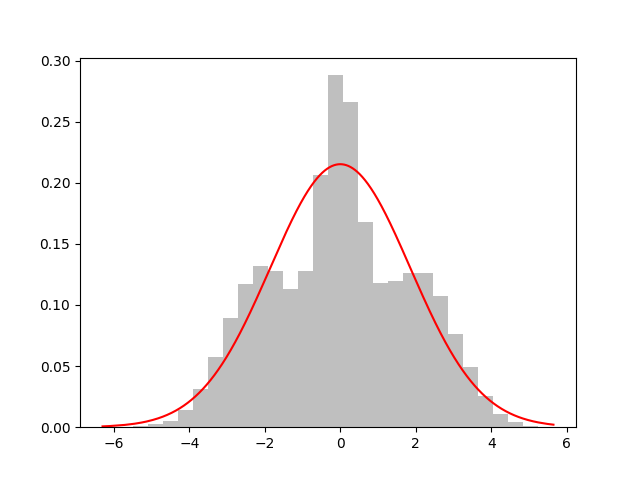
\includegraphics[width=1\linewidth]{../q1to6pics/q1.png}
			\caption{1 component Gaussian mixture model}
	\end{minipage}\hfill
\end{figure}
\pagebreak
\section{\MakeUppercase{Plot a 1,2, and 3 component Gaussian mixture model}}
As can be seen below, a two component mixture model clearly does a significantly better job than a single component mixture model, but the nature of the fit really only begins to be well represented when we have a component for each mean.
\begin{figure}[!htb]
	\centering
	\begin{minipage}{0.49\textwidth}
			\centering
			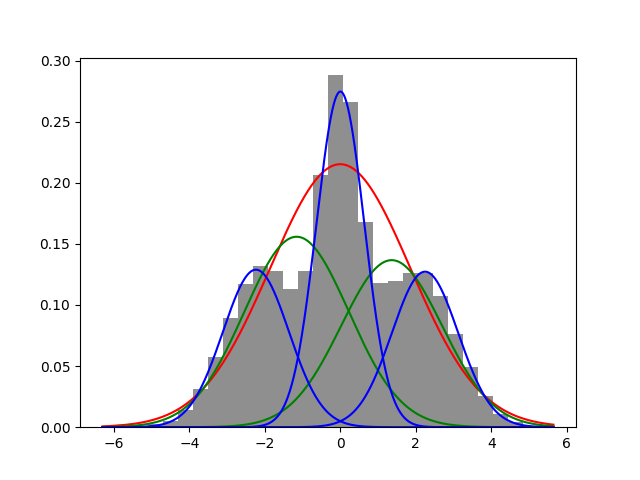
\includegraphics[width=1\linewidth]{../q1to6pics/q2.png}
			\caption{1, 2, and 3 component Gaussian mixture model}
	\end{minipage}\hfill
\end{figure}
\pagebreak
\section{\MakeUppercase{Plot a 1,2, and 4 component Gaussian mixture model}}
When comparing to the figure from the last section, we can see that having a fourth mixture component maintains the representation of a three component mixture model, but the change is small and the peak that is second from the left seems to just be subcomponent of the middle peak shown in a three component mixture model.
\begin{figure}[!htb]
	\centering
	\begin{minipage}{0.49\textwidth}
			\centering
			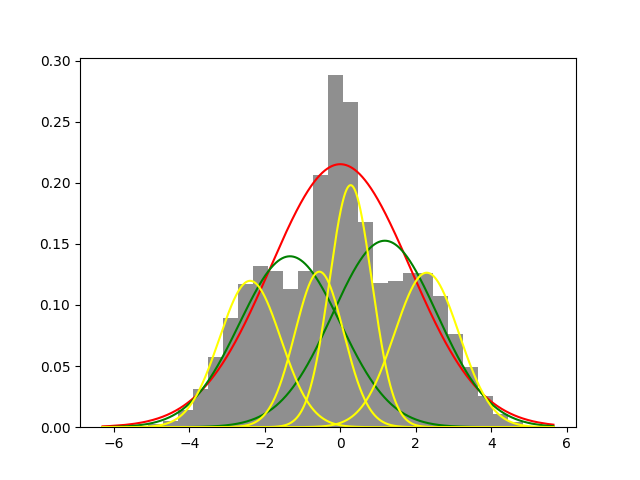
\includegraphics[width=1\linewidth]{../q1to6pics/q3.png}
			\caption{1, 2, and 4 component Gaussian mixture model}
	\end{minipage}\hfill
\end{figure}
\pagebreak
\section{\MakeUppercase{Plot the log probability of the data belong to n component Gaussian mixture models}}
As can be seen, the log likelihood of the data set peaks when the Gaussian mixture model has three components, but levels out afterwards. Since this dataset has 3 peaks, this is logical and we can see the rapid rise of log likelihood betweek one componenet and three components. 
\begin{figure}[!htb]
	\centering
	\begin{minipage}{0.49\textwidth}
			\centering
			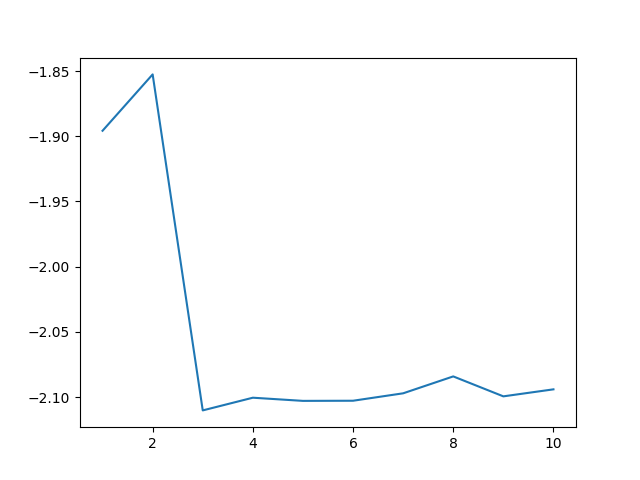
\includegraphics[width=1\linewidth]{../q1to6pics/q4.png}
			\caption{Log likelihood as a function of Gaussian mixture model components}
	\end{minipage}\hfill
\end{figure}
\section{\MakeUppercase{Summary}}
\end{document}